\documentclass{customDoc}
\usepackage{colortbl}
\usepackage{longtable}
\usepackage{booktabs}
\usepackage{gensymb}
\usepackage{longtable}
\usepackage{multirow}
\usepackage{graphicx}
\usepackage{subcaption}
\usepackage[per-mode=symbol]{siunitx}
\sisetup{detect-all}
\usepackage{multicol}
\usepackage{float}
\usepackage[inkscapelatex=false]{svg}
\usepackage{pstricks}

\begin{document}
\title{耦合摆实验 - 实验报告}
\class{トレセン学園 高等部二年生}
\name{アドマイヤベガ}
\id{1}

\maketitle

\section{摘要}

本实验探究了晶体的一些衍射性质,同时通过衍射图样反推出一些晶体的结构. 通过实验,了解到更多晶体学知识和衍射图样的分析方法.

\section{实验原理}

一束光入射二维晶格,若二维晶格的透过率函数为 $\rho(x,y)$,则

\begin{equation}
    F(q_x, q_y) = \int_{-x_0}^{x_0}\int_{-y_0}^{y_0} \rho(x,y)\exp[\text{i}(q_xx+q_yy)]\text{d}x\text{d}y
\end{equation}

这就是衍射图样的复振幅分布. 用 Fourier 变换可以反推晶体的晶胞结构,得到

\begin{equation}
    \rho(\vec{r}) \sim \int F(\vec{q})\exp(-\text{i}\vec{q}\cdot\vec{r})\text{d}\vec{q}
\end{equation}

对于离散的衍射斑,积分可以变成求和:

\begin{equation}
    \rho(\vec{r}) \sim \sum|F(\vec{q})|\exp(\text{i}\varphi)\exp(-\text{i}\vec{q}\cdot\vec{r})
\end{equation}

\section{实验仪器及实验步骤}

本实验使用台灯、激光笔、铬板 (内部有不同样品)、激光功率计、光屏、量角器和直尺.\newline


实验步骤如下:\newline


1. 观察一维样品的衍射图样,确定样品的 $q_1$ 和 $a$.

2. 观察二维样品的衍射图.

3. 探究晶体的对称性.

4. 通过相位的变化,确定晶体的完整结构.

\section{实验数据处理}

\subsection{一维样品}

样品 DG1 $\sim$ DG5 的衍射图样如下:

\begin{figure}[H]
    \begin{subfigure}[b]{0.45\textwidth}
        \includegraphics[width=\textwidth]{DG1.jpg}
        \caption{样品 DG1}
        \label{fig:1D_1}
    \end{subfigure}
    \hfill
    \begin{subfigure}[b]{0.45\textwidth}
        \includegraphics[width=\textwidth]{DG2.jpg}
        \caption{样品 DG2}
        \label{fig:1D_2}
    \end{subfigure}
    \\
    \begin{subfigure}[b]{0.45\textwidth}
        \includegraphics[width=\textwidth]{DG3.jpg}
        \caption{样品 DG3}
        \label{fig:1D_3}
    \end{subfigure}
    \hfill
    \begin{subfigure}[b]{0.45\textwidth}
        \includegraphics[width=\textwidth]{DG4.jpg}
        \caption{样品 DG4}
        \label{fig:1D_4}
    \end{subfigure}
    \\
    \begin{subfigure}[b]{0.45\textwidth}
        \includegraphics[width=\textwidth]{DG5.jpg}
        \caption{样品 DG5}
        \label{fig:1D_5}
    \end{subfigure}
    \caption{一维样品的衍射图样}
    \label{fig:1D}
\end{figure}

可以从图像中计算得到以下参数:

% Table generated by Excel2LaTeX from sheet 'Sheet1'
\begin{table}[H]
  \centering
    \begin{tabular}{|c|c|c|c|c|}
    \hline
    种类    & $\Delta x$ ($\si{\milli\metre}$) & $\theta$     &  $q_1$ ($\si{\metre}^{-1}$) & $a$ ($\si{\milli\metre}$) \\
    \hline
    DG1   & 14.7  & 0.032085 & 310254.6994 & 0.020251701 \\
    \hline
    DG2   & 5.8   & 0.012663 & 122413.4188 & 0.051327586 \\
    \hline
    DG3   & 3.8   & 0.008297 & 80201.89509 & 0.078342105 \\
    \hline
    DG4   & 3.6   & 0.00786 & 75980.74271 & 0.082694444 \\
    \hline
    DG5   & 3.4   & 0.007423 & 71759.59034 & 0.087558824 \\
    \hline
    \end{tabular}%
    \caption{一维样品衍射图样数据}
  \label{tab:1}%
\end{table}%

\subsection{二维样品}

观测样品 UC1 $\sim$ UC4 的衍射图样如下:

\begin{figure}[H]
    \begin{subfigure}[b]{0.45\textwidth}
        \includegraphics[width=\textwidth]{UC1.jpg}
        \caption{样品 UC1}
        \label{fig:2D_1}
    \end{subfigure}
    \hfill
    \begin{subfigure}[b]{0.45\textwidth}
        \includegraphics[width=\textwidth]{UC2.jpg}
        \caption{样品 UC2}
        \label{fig:2D_2}
    \end{subfigure}
    \\
    \begin{subfigure}[b]{0.45\textwidth}
        \includegraphics[width=\textwidth]{UC3.jpg}
        \caption{样品 UC3}
        \label{fig:2D_3}
    \end{subfigure}
    \hfill
    \begin{subfigure}[b]{0.45\textwidth}
        \includegraphics[width=\textwidth]{UC4.jpg}
        \caption{样品 UC4}
        \label{fig:2D_4}
    \end{subfigure}
    \caption{二维样品的衍射图样}
    \label{fig:2D}
\end{figure}

同上面一样,对二维样品也可以测量以下参数:

% Table generated by Excel2LaTeX from sheet 'Sheet1'
\begin{table}[H]
  \centering
    \begin{tabular}{|c|c|c|c|c|}
    \hline
    种类    & $\Delta x$ ($\si{\milli\metre}$) & $\theta$     &  $q_1$ ($\si{\metre}^{-1}$) & $a$ ($\si{\milli\metre}$) \\
    \hline
    UC1   & 9.7   & 0.021176 & 204725.8901 & 0.030690722 \\
    \hline
    UC2   & 14.4  & 0.031431 & 303922.9709 & 0.020673611 \\
    \hline
    UC3   & 21.9  & 0.04778 & 462216.1848 & 0.013593607 \\
    \hline
    UC4   & 9.4   & 0.020521 & 198394.1615 & 0.031670213 \\
    \hline
    \end{tabular}%
    \caption{二维样品衍射图样数据}
  \label{tab:2}%
\end{table}%

可以比较不同样品和讲义中的晶胞单元的对应关系:\newline


UC1:B,UC2:A,UC3:D,UC4:C.\newline


理由:UC3 为 D,因为它的图像出现缺级;D 的简单晶胞可视为 A 旋转 $45$ 度后拉长 $\sqrt{2}$ 倍,将 UC3 旋转 $45$ 度后与其余图案相似;UC2 的晶胞常数最小,UC1 与 UC4 相近,而 B 的晶胞常数大于 A,故 UC2 为 A;UC1 与 UC4 相比 UC1 的 0 级斑更亮,而讲义中的 C 透光率不如 B,零级斑更加暗,故 UC1 为 B,UC4 为 C.\newline


样品 UC5 $\sim$ UC7 的晶格结构更为复杂,其衍射图样如下:

\begin{figure}[H]
    \begin{subfigure}[b]{0.45\textwidth}
        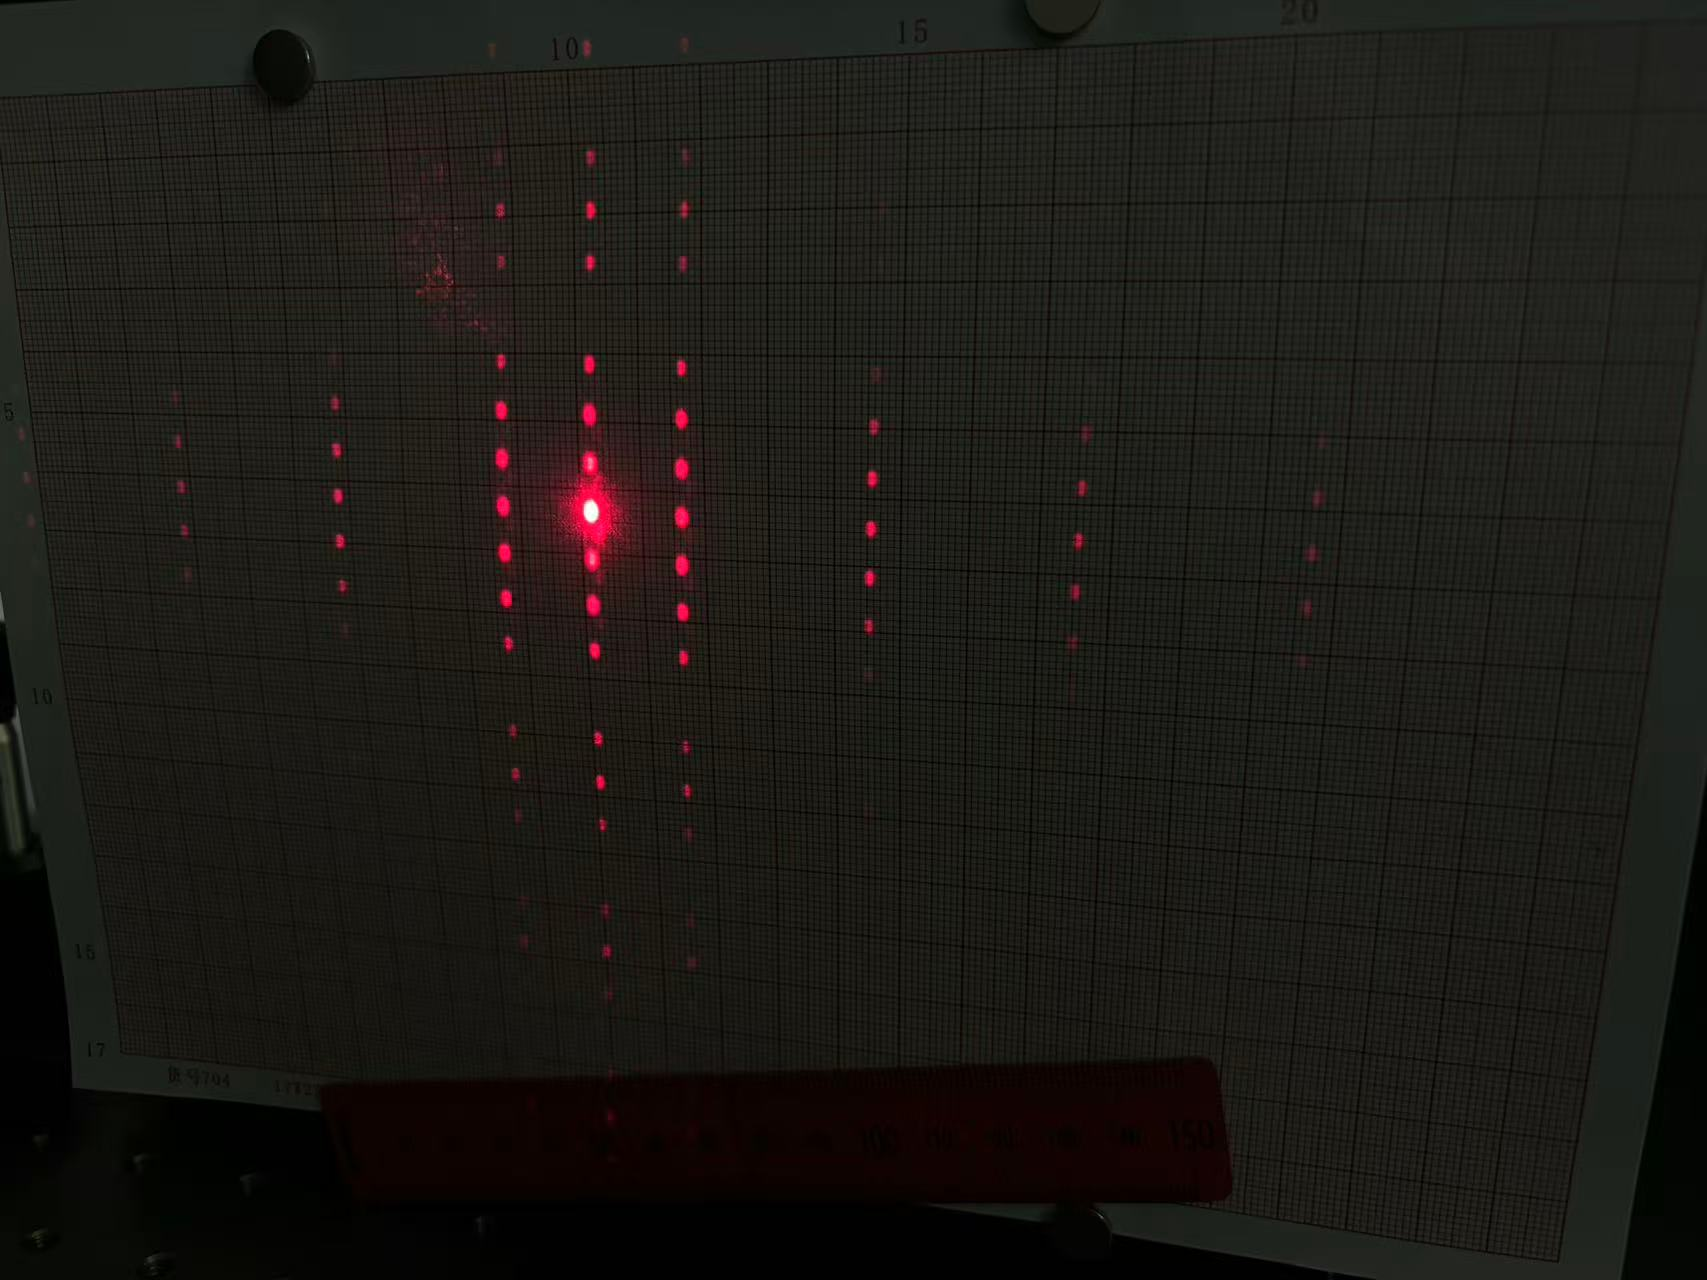
\includegraphics[width=\textwidth]{UC5.jpg}
        \caption{样品 UC5}
        \label{fig:2D_5}
    \end{subfigure}
    \hfill
    \begin{subfigure}[b]{0.45\textwidth}
        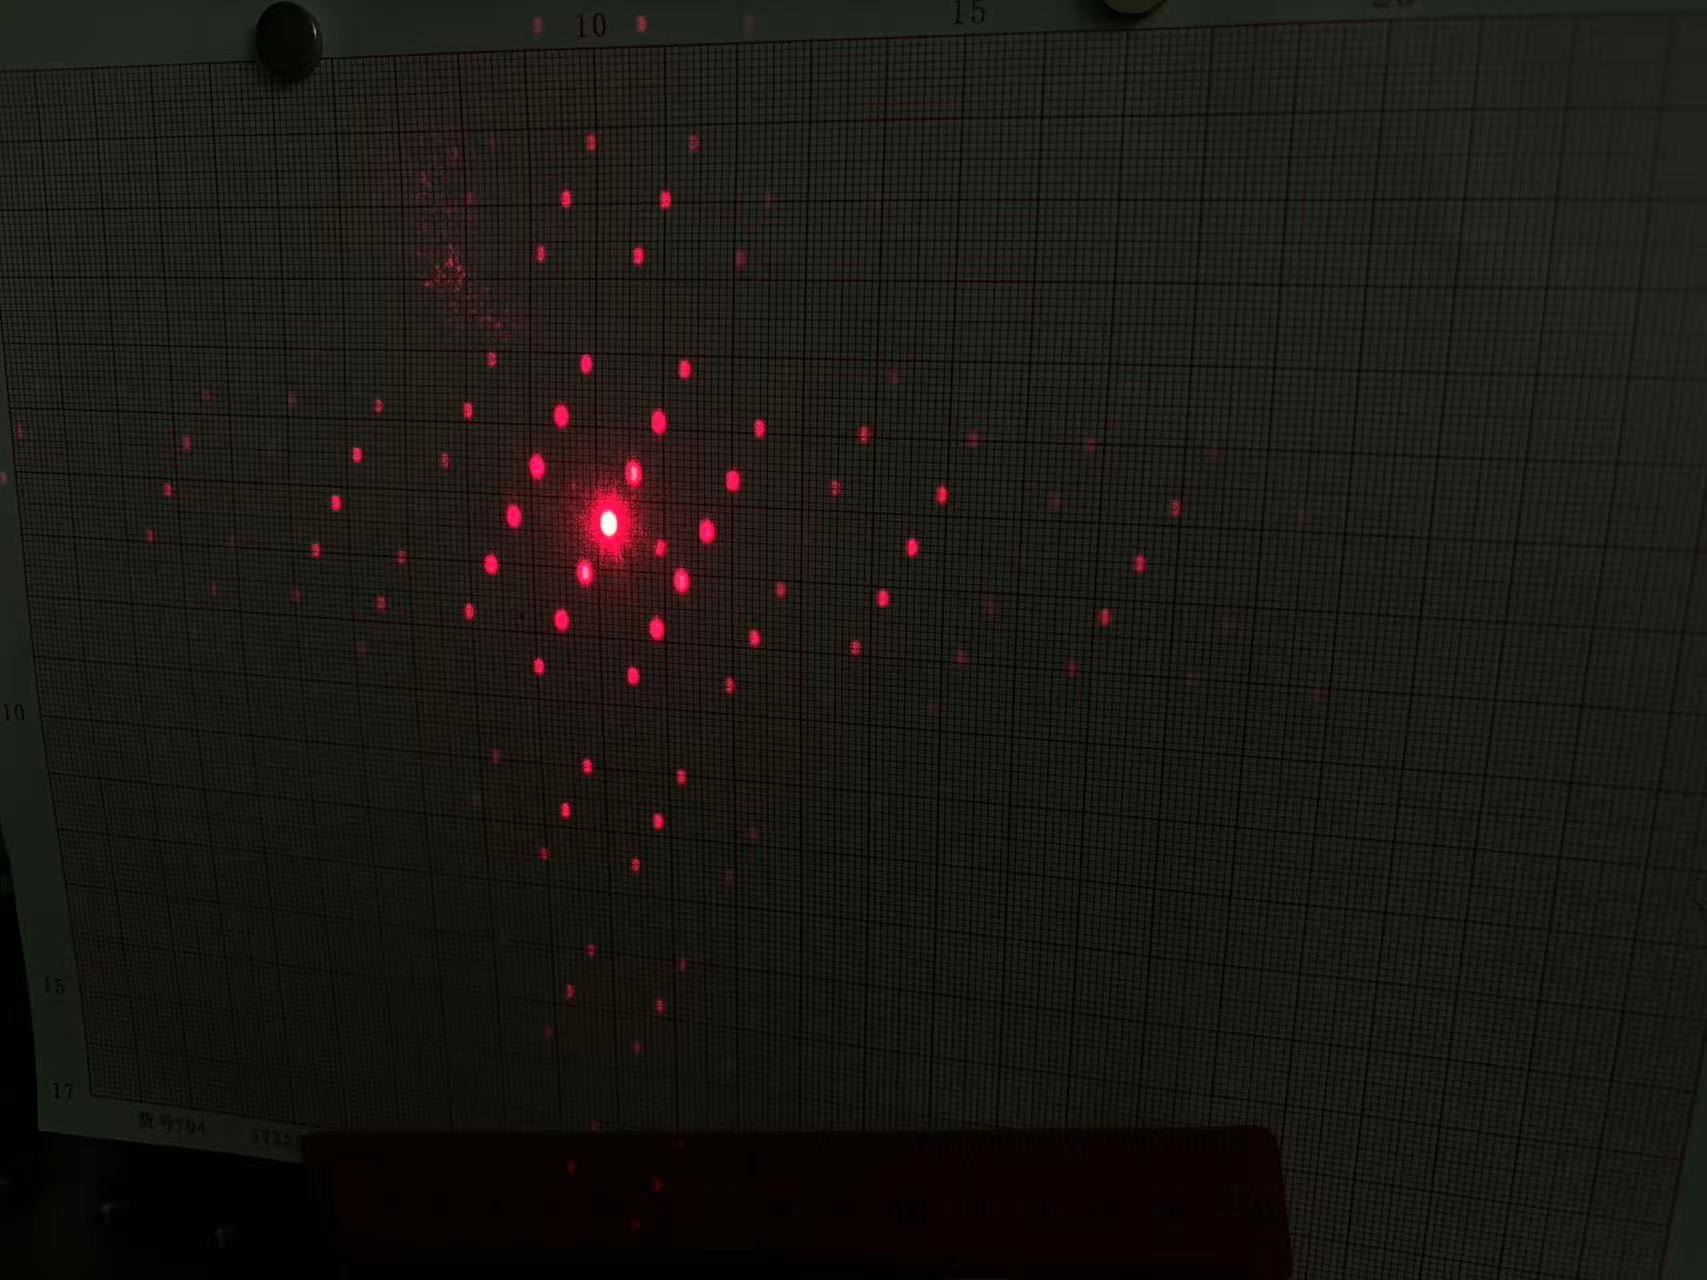
\includegraphics[width=\textwidth]{UC6.jpg}
        \caption{样品 UC6}
        \label{fig:2D_6}
    \end{subfigure}
    \\
    \begin{subfigure}[b]{0.45\textwidth}
        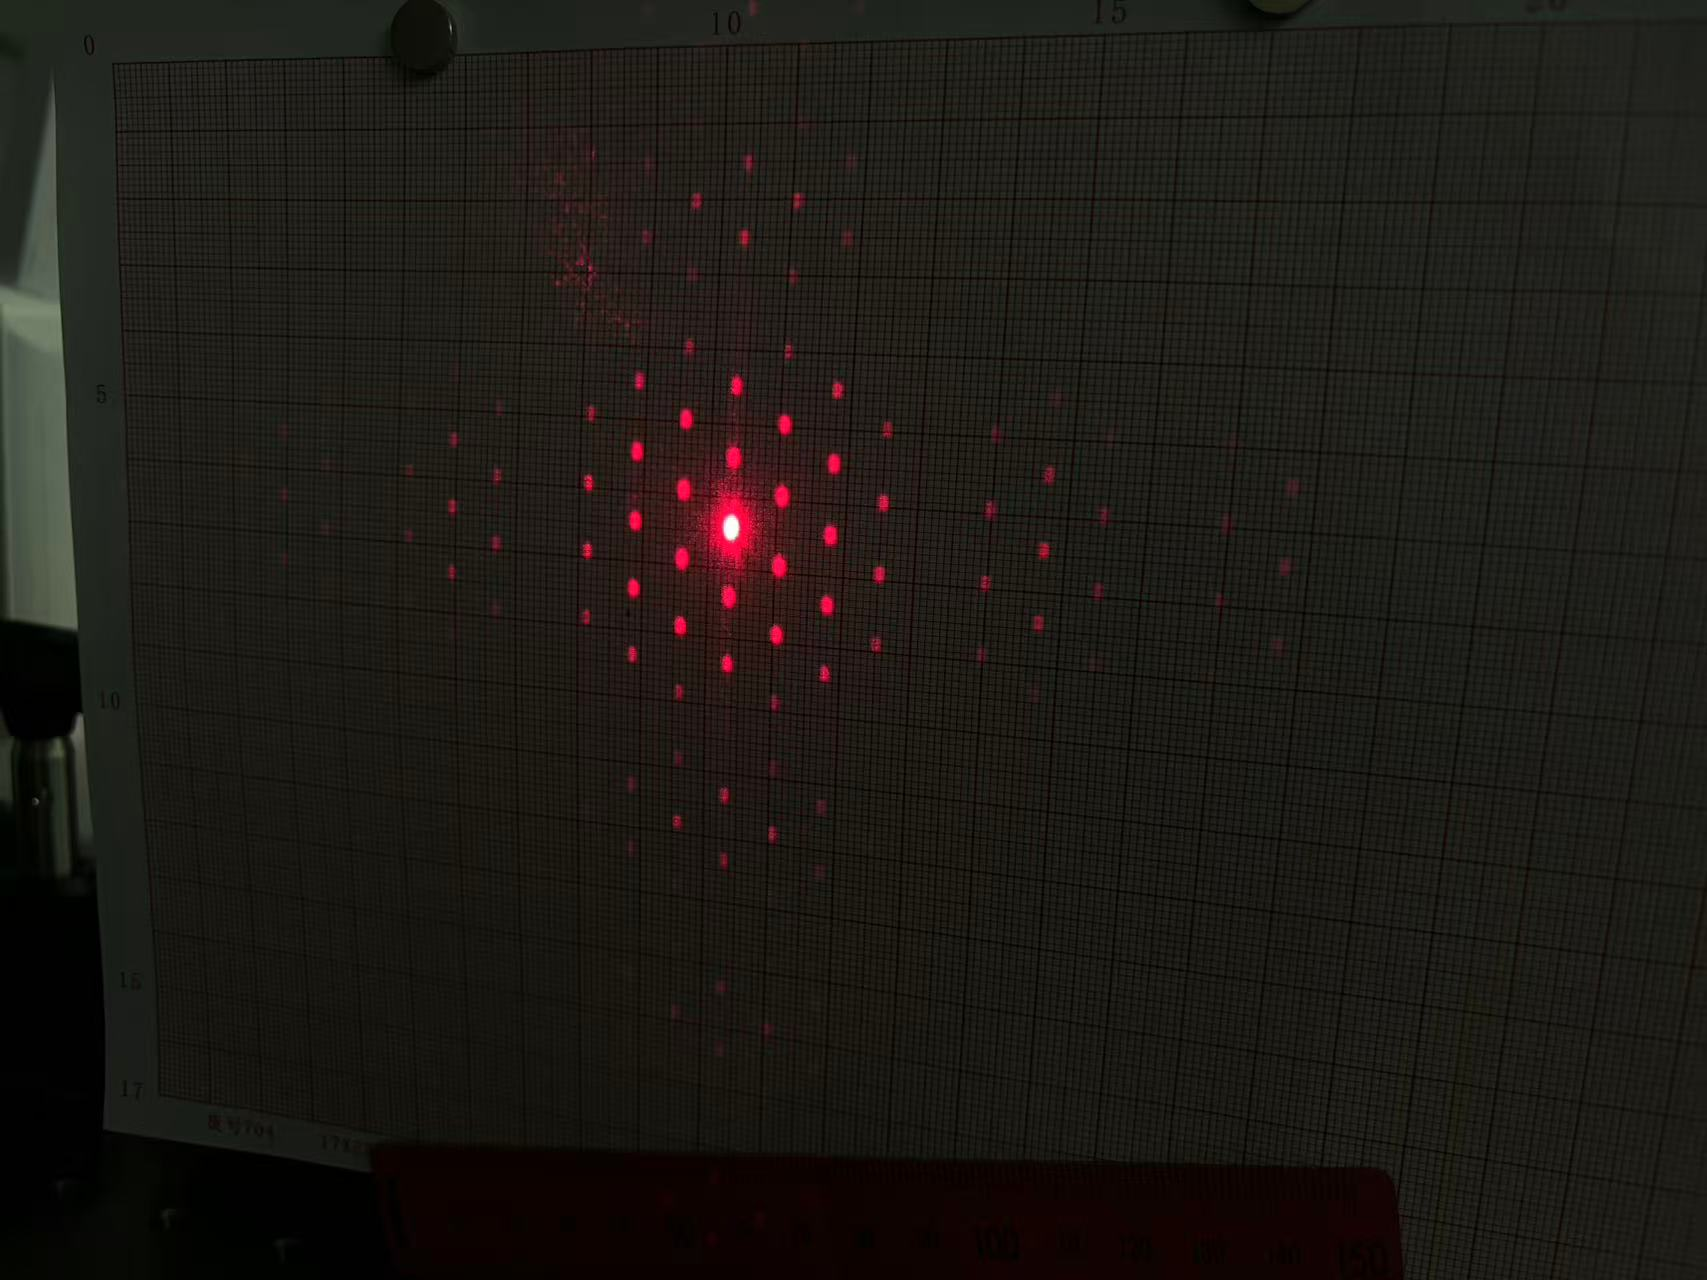
\includegraphics[width=\textwidth]{UC7.jpg}
        \caption{样品 UC7}
        \label{fig:2D_7}
    \end{subfigure}
    \caption{二维样品的衍射图样 (复杂)}
    \label{fig:2D_complex}
\end{figure}

分别得到这样的数据:

% Table generated by Excel2LaTeX from sheet 'Sheet1'
\begin{table}[H]
  \centering
    \begin{tabular}{|c|c|c|c|c|c|}
    \hline
    种类    & $\Delta x_1$ ($\si{\milli\metre}$) & $\Delta x_2$ ($\si{\milli\metre}$) & $\alpha$     & $a_1$ ($\si{\milli\metre}$) & $a_2$ ($\si{\milli\metre}$) \\
    \hline
    UC5   & 19    & 8     & 1.570796327 & 0.015668421 & 0.0372125 \\
    \hline
    UC6   & 12.21 & 8.06  & 1.626469888 & 0.024419489 & 0.036992799 \\
    \hline
    UC7   & 8.6   & 8.3   & 1.122706639 & 0.038408062 & 0.039796305 \\
    \hline
    \end{tabular}%
    \caption{二维样品衍射图样数据 (复杂)}
  \label{tab:3}%
\end{table}%

\subsection{探究晶体对称性}

讲义中所示的几种晶胞结构的对称性如下:

\begin{figure}[H]
    \begin{subfigure}[b]{0.2\textwidth}
        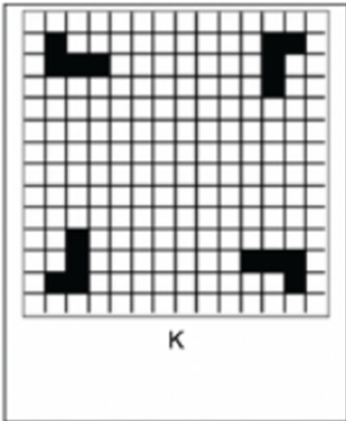
\includegraphics[width=\textwidth]{K.png}
        \caption{$C_1,C_2,C_4$ 对称}
        \label{fig:symmetry_A}
    \end{subfigure}
    \hfill
    \begin{subfigure}[b]{0.2\textwidth}
        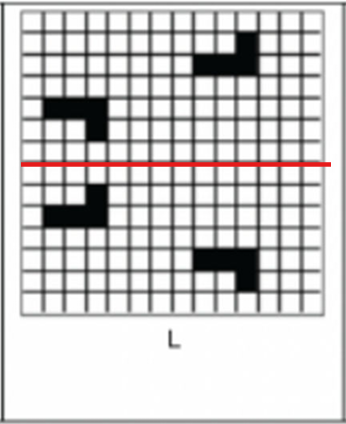
\includegraphics[width=\textwidth]{L.png}
        \caption{镜像对称}
        \label{fig:symmetry_B}
    \end{subfigure}
    \hfill
    \begin{subfigure}[b]{0.2\textwidth}
        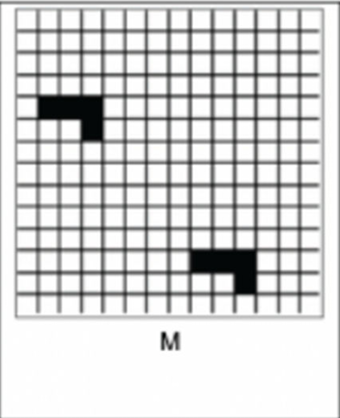
\includegraphics[width=\textwidth]{M.png}
        \caption{$C_1$ 对称}
        \label{fig:symmetry_C}
    \end{subfigure}
    \hfill
    \begin{subfigure}[b]{0.2\textwidth}
        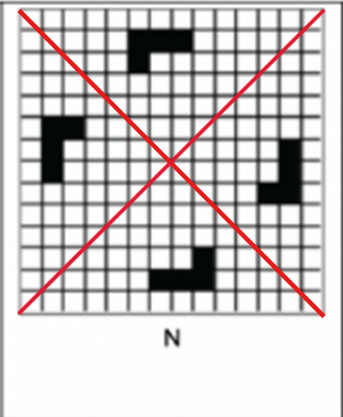
\includegraphics[width=\textwidth]{N.png}
        \caption{$C_1,C_2$,镜像对称}
        \label{fig:symmetry_D}
    \end{subfigure}
    \caption{晶胞的对称性分析}
    \label{fig:symmetry_analysis}
\end{figure}

样品 PG1、2、5、8 的衍射图样如图所示:

\begin{figure}[H]
    \begin{subfigure}[b]{0.45\textwidth}
        \includegraphics[width=\textwidth]{PG1.jpg}
        \caption{样品 PG1}
        \label{fig:symmetry_1}
    \end{subfigure}
    \hfill
    \begin{subfigure}[b]{0.45\textwidth}
        \includegraphics[width=\textwidth]{PG2.jpg}
        \caption{样品 PG2}
        \label{fig:symmetry_2}
    \end{subfigure}
    \\
    \begin{subfigure}[b]{0.45\textwidth}
        \includegraphics[width=\textwidth]{PG5.jpg}
        \caption{样品 PG5}
        \label{fig:symmetry_3}
    \end{subfigure}
    \hfill
    \begin{subfigure}[b]{0.45\textwidth}
        \includegraphics[width=\textwidth]{PG8.jpg}
        \caption{样品 PG8}
        \label{fig:symmetry_4}
    \end{subfigure}
    \caption{晶胞的对称性分析}
    \label{fig:symmetry_analysis_complex}
\end{figure}

从衍射图样的对称性,可以将讲义上的晶胞结构与样品进行对应:\newline


PG1:L,PG2:M,PG5:N,PG8:K.\newline


一个特殊的样品是 UC8,它的衍射图样如下:

\begin{figure}[H]
    \centering
    \includegraphics[width=0.45\textwidth]{UC8.jpg}
    \caption{样品 UC8}
    \label{fig:UC8}
\end{figure}

这个图样具有 $C_{10}$ 对称性,说明它不可能是一个晶体.

\subsection{探究相位问题}

下面是样品 MR1 的衍射图样:

\begin{figure}[H]
    \centering
    \includegraphics[width=0.45\textwidth]{MR1.jpg}
    \caption{样品 MR1}
    \label{fig:MR1}
\end{figure}

以及光度数据:

% Table generated by Excel2LaTeX from sheet 'Sheet1'
\begin{table}[H]
  \centering
    \begin{tabular}{|r|c|c|c|c|c|l|}
    \hline
    \textbf{(k)} &       &       &       &       &       &  \\
    \hline
    \textbf{2} & \multicolumn{1}{r|}{8.0} & \multicolumn{1}{r|}{36.7} & \multicolumn{1}{r|}{1.3} & \multicolumn{1}{r|}{31.7} & \multicolumn{1}{r|}{7.9} &  \\
    \hline
    \textbf{1} & \multicolumn{1}{r|}{38.9} & \multicolumn{1}{r|}{28.9} & \multicolumn{1}{r|}{20.3} & \multicolumn{1}{r|}{1.2} & \multicolumn{1}{r|}{37.2} &  \\
    \hline
    \textbf{0} & \multicolumn{1}{r|}{1.5} & \multicolumn{1}{r|}{17.9} & \multicolumn{1}{r|}{319.7} & \multicolumn{1}{r|}{21.4} & \multicolumn{1}{r|}{1.1} &  \\
    \hline
    \textbf{-1} & \multicolumn{1}{r|}{35.2} & \multicolumn{1}{r|}{28.3} & \multicolumn{1}{r|}{21.4} & \multicolumn{1}{r|}{1.3} & \multicolumn{1}{r|}{34.9} &  \\
    \hline
    \textbf{-2} & \multicolumn{1}{r|}{8.3} & \multicolumn{1}{r|}{35.8} & \multicolumn{1}{r|}{0.9} & \multicolumn{1}{r|}{34.2} & \multicolumn{1}{r|}{3.8} &  \\
    \hline
          & \textbf{-2} & \textbf{-1} & \textbf{0} & \textbf{1} & \textbf{2} & \textbf{(h)} \\
    \hline
    \end{tabular}%
    \caption{晶体各衍射斑点强度测试值}
  \label{tab:4}%
\end{table}%

可以迭代计算得到透射率的分布:

% Table generated by Excel2LaTeX from sheet 'Sheet1'
\begin{table}[H]
  \centering
    \begin{tabular}{|r|c|c|c|c|l|}
    \hline
    $(\gamma)$ &       &       &       &       &  \\
    \hline
    \textbf{3} & \multicolumn{1}{r|}{4.108} & \multicolumn{1}{r|}{12.971} & \multicolumn{1}{r|}{27.528} & \multicolumn{1}{r|}{-14.119} &  \\
    \hline
    \textbf{2} & \multicolumn{1}{r|}{2.338} & \multicolumn{1}{r|}{62.810} & \multicolumn{1}{r|}{-28.079} & \multicolumn{1}{r|}{59.128} &  \\
    \hline
    \textbf{1} & \multicolumn{1}{r|}{1.789} & \multicolumn{1}{r|}{40.969} & \multicolumn{1}{r|}{42.525} & \multicolumn{1}{r|}{-9.439} &  \\
    \hline
    \textbf{0} & \multicolumn{1}{r|}{54.185} & \multicolumn{1}{r|}{-0.707} & \multicolumn{1}{r|}{0.460} & \multicolumn{1}{r|}{9.617} &  \\
    \hline
          & \textbf{0} & \textbf{1} & \textbf{2} & \textbf{3} & $(\chi)$ \\
    \hline
    \end{tabular}%
    \caption{晶胞的振幅透射率}
  \label{tab:addlabel}%
\end{table}%

与讲义中的选项进行对比,可以得到晶格应该为 X.

\section{分析与讨论}

手机拍摄的衍射图样中经常出现另一组点,这可能是因为样品在铬板上有一定厚度,所以产生了反射.

\section{原始数据截图}

\begin{figure}[H]
    \centering
    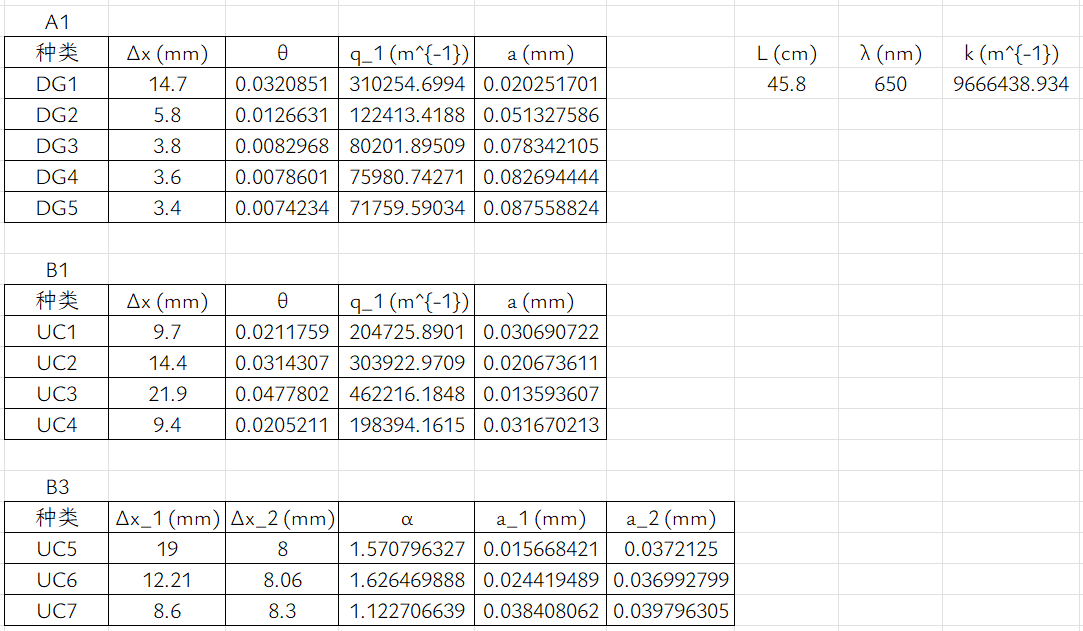
\includegraphics[width=\textwidth]{originData-1.png}
    \caption{原始数据截图 (1)}
    \label{fig:data1}
\end{figure}
\begin{figure}[H]
    \centering
    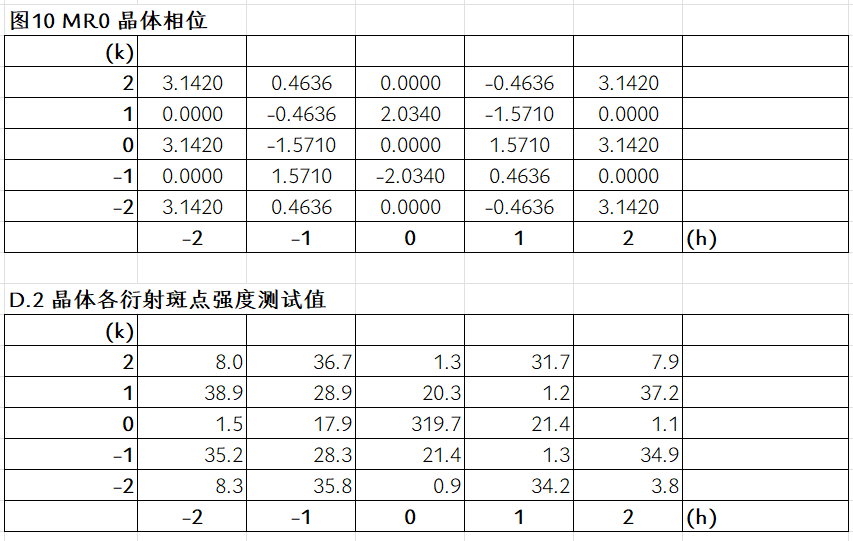
\includegraphics[width=\textwidth]{originData-2.png}
    \caption{原始数据截图 (2)}
    \label{fig:data2}
\end{figure}
\begin{figure}[H]
    \centering
    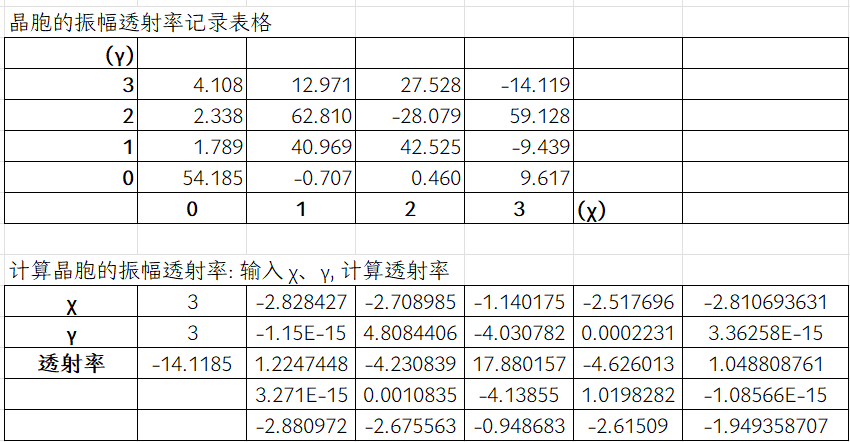
\includegraphics[width=\textwidth]{originData-3.png}
    \caption{原始数据截图 (3)}
    \label{fig:data3}
\end{figure}

\end{document}